\documentclass{article}
\usepackage[utf8]{inputenc}
\usepackage{geometry}
\usepackage{graphicx}
\usepackage{graphics}
\geometry{total={210mm,297mm},
left=25mm,right=25mm,%
bindingoffset=0mm, top=20mm,bottom=20mm}
\title{LaTeX}
\date{2020}


\begin{document}

\section*{GNUplot}

\subsection*{Cumulative distribution function}
$\text{(https://en.wikipedia.org/wiki/Normal\_distribution)}$
\newline
The cumulative distribution function (CDF) of the standard normal distibution, usually denoted with the capital Greek letter $\Phi$ (phi), is the integral $$ \Phi(x)=\frac{1}{\sqrt{2 \pi}} \int_{-\infty}^{x} e^{-t^{2} / 2} d t $$ The related error function erf( $(x)$ gives the probability of a random variable with normal distribution of mean 0 and variance 1/2 falling in the range $[-x, x]$; that is $$ {erf}(x)=\frac{2}{\sqrt{\pi}} \int_{0}^{x} e^{-t^{2}} d t $$ These integrals cannot be expressed in terms of elementary functions, and are often said to be special functions. However, many numerical approximations are known; see below. The two functions are closely related, namely $$ \Phi(x)=\frac{1}{2}\left[1+{erf}\left(\frac{x}{\sqrt{2}}\right)\right] $$ For a generic normal distribution with density $f$, mean $\mu$ and deviation $\sigma$, the cumulative distribution function is $$ F(x)=\Phi\left(\frac{x-\mu}{\sigma}\right)=\frac{1}{2}\left[1+{erf}\left(\frac{x-\mu}{\sigma \sqrt{2}}\right)\right] $$
\begin{figure}[h]
	\centering
	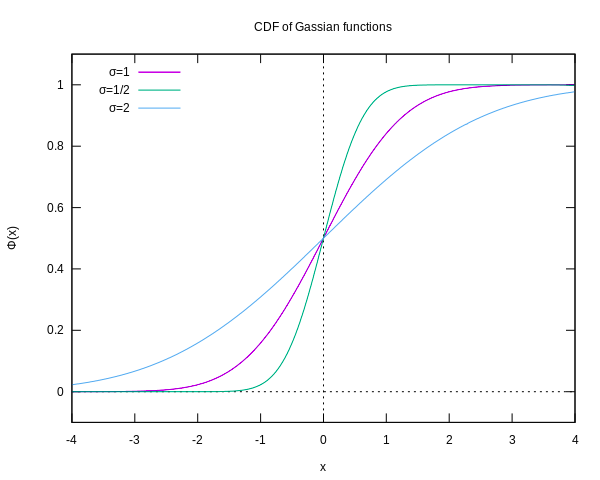
\includegraphics[width=0.7\linewidth]{CDF}
	\caption{}
	\label{fig:cdf}
\end{figure}
 
\end{document}
